\documentclass[conference]{IEEEtran}

% Pacotes para suporte ao Português e imagens
\usepackage[utf8]{inputenc}
\usepackage[T1]{fontenc}
\usepackage[brazilian]{babel}
\usepackage{amsmath,amssymb,amsfonts}
\usepackage{algorithmic}
\usepackage{graphicx}
\usepackage{textcomp}
\usepackage{xcolor}

\begin{document}

\title{Relatório de Práticas em Sistemas Digitais - Laboratórios 01 e 02}

\author{\IEEEauthorblockN{Lucca, João Vital, Danyel}
\IEEEauthorblockA{\textit{Departamento de Computação (DCOMP)} \\
\textit{Universidade Federal de Sergipe (UFS)}\\
São Cristóvão, Brasil \\
}
}

\maketitle

\begin{abstract}
Este relatório descreve as atividades práticas conjuntas realizadas nos Laboratórios 01 e 02. A primeira parte foca na operação de instrumentos de bancada e na análise da dinâmica temporal de circuitos Resistor/Capacitor (RC), avaliando efeitos de carga e limites de frequência (full swing). A segunda parte aborda a compreensão e comparação estrutural entre as famílias lógicas TTL (Transistor-Transistor Logic) e CMOS (Complementary Metal-Oxide Semiconductor), incluindo a leitura de datasheets, limites operacionais e a montagem de inversores lógicos. O estudo integrado estabelece a relação entre as limitações analógicas temporais e a implementação física das portas lógicas digitais.
\end{abstract}

\begin{IEEEkeywords}
Sistemas Digitais, Instrumentação, Circuito RC, CMOS, TTL, Inversores, Datasheet.
\end{IEEEkeywords}

% ==========================================
% LABORATÓRIO 01
% ==========================================
\section{Laboratório 01: Instrumentação e Circuito RC}

\subsection{Introdução Teórica}
Os sistemas digitais diferem dos analógicos por manipularem grandezas de forma discreta (níveis lógicos 0 e 1), enquanto os analógicos operam com valores contínuos. Apesar dessa abstração perfeita, o hardware que implementa essas lógicas reside no mundo analógico. Para compreender limitações físicas, como tempos de atraso e de transição de sinal, é fundamental analisar o comportamento de cargas e descargas de capacitores em malhas RC. Além disso, tecnologias modernas, como a família CMOS, destacam-se por possuir consumo estático quase nulo, consumindo corrente predominantemente durante o chaveamento das capacitâncias parasitas e de carga.

\subsection{Materiais Utilizados}
\begin{itemize}
    \item \textbf{Instrumentos de bancada:} Protoboard, multímetro, osciloscópio, gerador de funções e fonte de tensão contínua.
    \item \textbf{Componentes passivos:} Fios de ligação, LEDs e resistores variados.
    \item \textbf{Capacitores:} 2.2 pF, 10 nF e 100 nF.
\end{itemize}

\subsection{Descrição das Atividades e Resultados}

\subsubsection{Instrumentação e Adaptação à Protoboard}
A atividade inicial consistiu na montagem de um circuito simples com LED alimentado por uma fonte contínua. Ao medir o resistor limitador com o multímetro, observou-se uma variação percentual em relação ao valor nominal do código de cores. Essa diferença ocorre pelas tolerâncias de fabricação (geralmente de 5\% a 10\%), confirmando as imperfeições do mundo físico em relação ao modelo ideal.

\subsubsection{Circuito RC e Dinâmica Temporal}
Montou-se um circuito RC excitado por uma fonte variável (gerador de onda quadrada). Ao substituir o capacitor de 10 nF por um de 100 nF, os tempos de transição (subida de 10\% a 90\% e descida de 90\% a 10\%) aumentaram drasticamente no osciloscópio.

\paragraph{Justificativa e Frequência de Full Swing}
A tensão no capacitor obedece à equação de carga regida pela constante $\tau = R \cdot C$. Com um capacitor de 100 nF, o circuito exige mais tempo para atingir a tensão máxima. Consequentemente, a frequência máxima suportada diminui. Se a frequência for muito alta, a onda inverte o pulso antes da carga completa, impedindo o \textit{full swing} (transição total entre $V_{DD}$ e GND).

\paragraph{Consumo Dinâmico (Análogo ao CMOS)}
A análise da corrente no osciloscópio revelou picos pontuais que ocorrem unicamente nos instantes de mudança de estado da onda quadrada. Conclui-se que o consumo na tecnologia CMOS ocorre predominantemente durante o chaveamento para carregar/descarregar a rede.

\subsection{Conclusões do Laboratório 01}
Ficou evidente que a construção de sistemas digitais depende do domínio de fenômenos analógicos. As transições lógicas não são instantâneas; as capacitâncias da rede governam os tempos de subida e descida. A velocidade e o desempenho do circuito são severamente limitados pelo tempo físico de carga/descarga dos nós, e a visualização dos picos de corrente elucidou o benefício do baixo consumo estático da tecnologia CMOS.

% ==========================================
% LABORATÓRIO 02
% ==========================================
\section{Laboratório 02: Famílias Lógicas e Inversores}

\subsection{Introdução Teórica}
A porta lógica é o bloco fundamental que implementa a Álgebra Booleana no hardware. Historicamente, a tecnologia TTL, baseada em transistores bipolares (BJT), foi o padrão, mas foi substituída pela CMOS. Esta última utiliza pares complementares de MOSFETs (canal P e N), suportando faixas de alimentação amplas, operando com altíssima impedância de entrada e consumo estático mínimo. Para a montagem correta, a análise prévia dos \textit{datasheets} é obrigatória para verificar pinagens e tensões máximas.

\subsection{Materiais Utilizados}
\begin{itemize}
    \item \textbf{Instrumentos:} Protoboard, multímetro, fonte contínua, fios e LEDs.
    \item \textbf{Circuitos Integrados (CIs):} TTL 74LS04 (Inversor Sêxtuplo) e CMOS CD4007 (Inversor a partir de transistores MOS discretos).
    \item \textbf{Documentação:} \textit{Datasheets} dos CIs.
\end{itemize}

\subsection{Descrição das Atividades e Resultados}

\subsubsection{Características Típicas e Limites de Operação}
A leitura dos manuais revelou diferenças críticas:
\begin{itemize}
    \item \textbf{TTL (74LS04):} Exige tensão nominal em torno de 5V e opera com margens estreitas de reconhecimento (entradas $\le 0,8$V para nível BAIXO e $\ge 2,0$V para nível ALTO).
    \item \textbf{CMOS (CD4007):} Tolera faixas amplas (3V a 15V), com limiares de reconhecimento atrelados à tensão de $V_{DD}$ escolhida.
\end{itemize}
As operações em bancada respeitaram rigorosamente estes limites para evitar danos térmicos.

\subsubsection{Inversores TTL e CMOS}
Montou-se um inversor usando a porta do 74LS04, acoplada a um LED. O sinal foi invertido perfeitamente. Posteriormente, implementou-se o inversor de forma estrutural conectando os transistores NMOS e PMOS do CI CD4007.

\paragraph{Estrutura e Leiaute da Porta NOT CMOS}
Comprovou-se que a tecnologia CMOS necessita de menos componentes periféricos que a TTL. O leiaute exigiu as seguintes conexões: portas (\textit{gates}) unidas para a entrada, fonte do PMOS no $+V_{DD}$, fonte do NMOS no GND, e os drenos (\textit{drains}) unidos para a saída invertida.

\subsection{Conclusões do Laboratório 02}
A manipulação dos componentes expôs as distinções de fabricação. Enquanto o TTL exige margens rigorosas de corrente e alimentação, o CMOS proporciona alta impedância de entrada e consumo estático insignificante. A montagem estrutural no CD4007 consolidou a leitura de datasheets e demonstrou a simplicidade geométrica da porta lógica, explicando a facilidade de integração em larga escala (LSI e VLSI) da tecnologia CMOS.

\begin{figure}[htbp]
\centerline{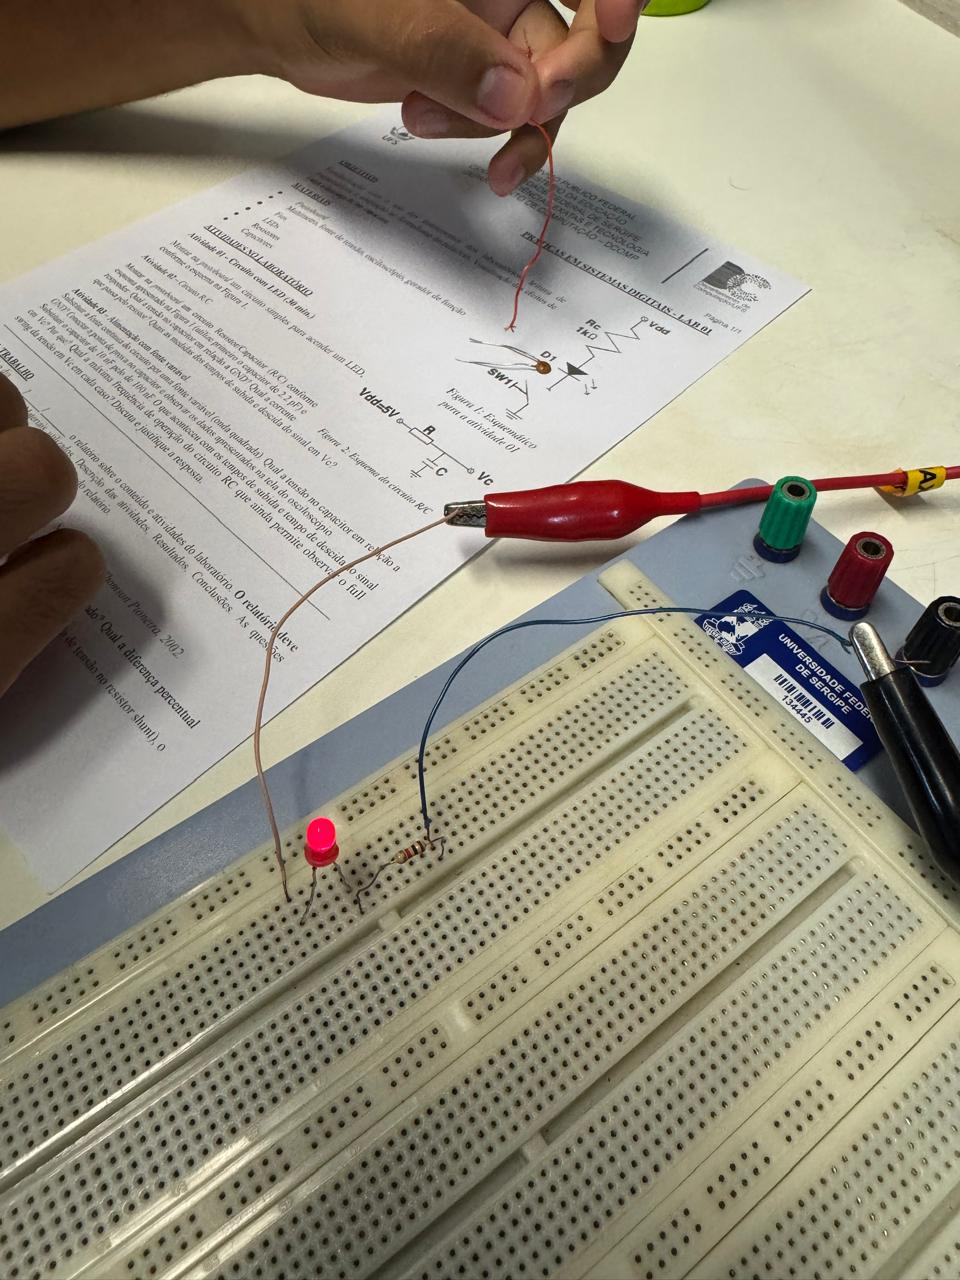
\includegraphics[width=0.7\columnwidth]{1.jpeg}}
\caption{Circuito básico montado em protoboard com o LED aceso.}
\label{fig1}
\end{figure}


\begin{figure}[htbp]
\centerline{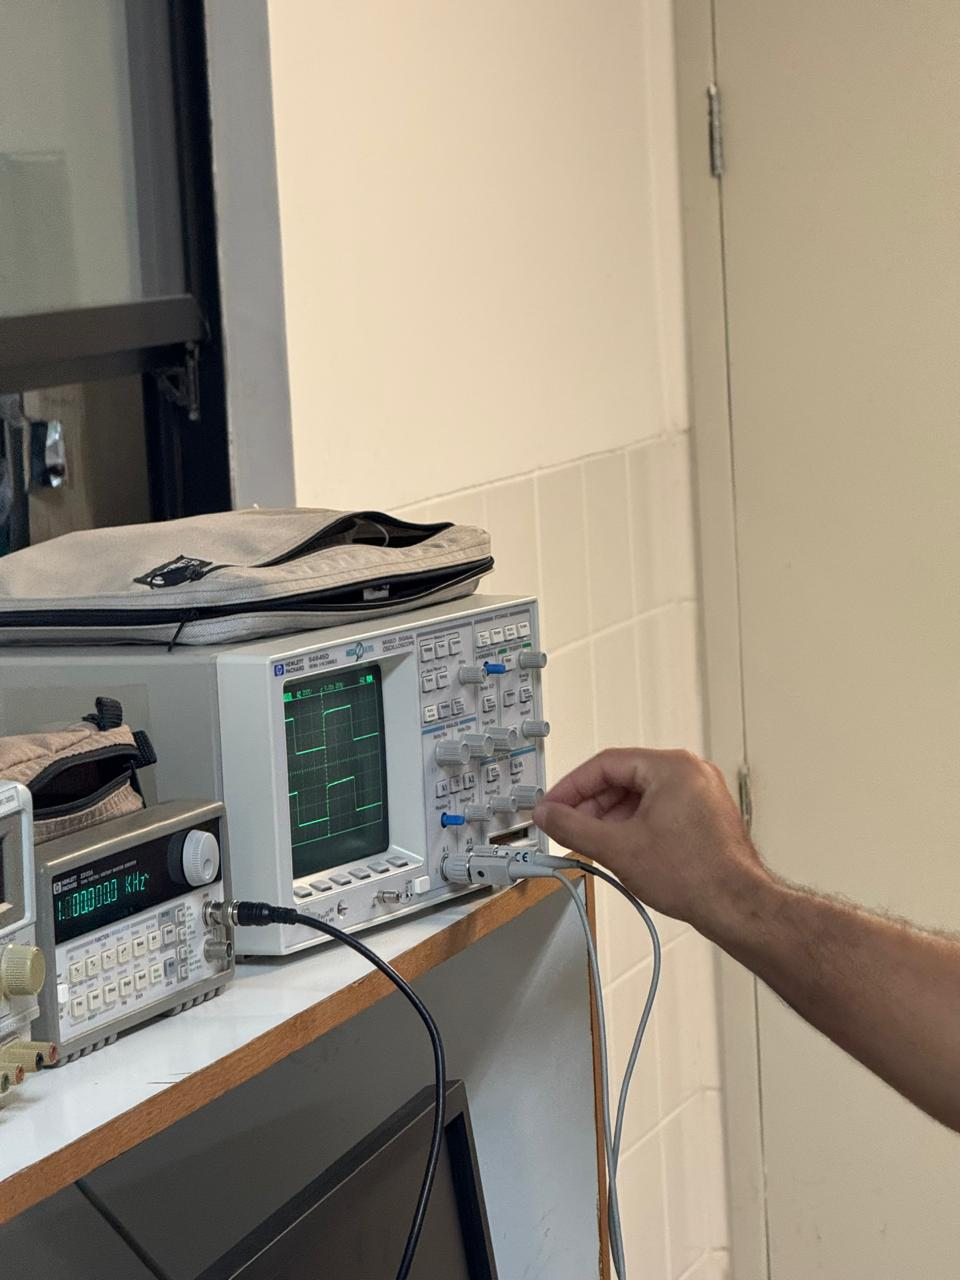
\includegraphics[width=0.7\columnwidth]{2.jpeg}}
\caption{Visualização do osciloscópio.}
\label{fig2}
\end{figure}

% ==========================================
% REFERÊNCIAS
% ==========================================
\begin{thebibliography}{00}
\bibitem{b1} R. A. L. Reis, \textit{Concepção de Circuitos Integrados}. Porto Alegre: Bookman, 2009.
\bibitem{b2} J. P. Uyemura, \textit{Sistemas digitais: uma abordagem integrada}. São Paulo: Thomson/Pioneira, 2002.
\bibitem{b3} R. Tocci, N. Widmer, and G. Moss, \textit{Sistemas Digitais - Princípios e Aplicações}, 12th ed. São Paulo: Pearson, 2018.
\end{thebibliography}

\end{document}
